\section{Experiments}
\label{sec:experiments}
In this section, extensive experiments are conducted to verify the effectiveness and superiority of the proposed MS-GAT\footnote{The code is available at: \url{https://github.com/luokn/ms-gat}.}.

\subsection{Experiment setup}
\subsubsection{Data description}
We evaluate the performance of MS-GAT on five public traffic network datasets: the PEMS-BAY dataset  \cite{li2017diffusion} and the PEMSD3, PEMSD4, PEMSD7 and PEMSD8 datasets  \cite{song2020spatial}. They were all constructed from the Caltrans Performance Measurement System (PeMS) \cite{chen2001freeway} and are commonly used in traffic prediction. Each of these five datasets is associated with a district of California, i.e., corresponding to a separate traffic road network, respectively. All time-series readings in these datasets are aggregated into 5-minute windows, which means there are 12 sampling points (i.e., timesteps) for every hour. Table I shows the related information of the five datasets. Note that, PEMSD4, PEMSD8 and PEMS-BAY contain three kinds of traffic signals (indicators) at each node: traffic flow, average speed and average occupancy, whereas PEMSD3 and PEMSD7 just involve the traffic flow.

\begin{table}[!htb]
    \caption{The Data description and statistics.}
    \label{tab:datasets}
    \centering
    \begin{tabular}{ccccc}
        \toprule[2pt]
        Datasets & \#Nodes & \#Edges & \#TimeSteps & \#Channels \\
        \hline
        PEMSD3   & 358     & 547     & 26208       & 1          \\
        PEMSD4   & 307     & 340     & 16992       & 3          \\
        PEMSD7   & 883     & 866     & 28224       & 1          \\
        PEMSD8   & 170     & 295     & 17856       & 3          \\
        PEMS-BAY & 325     & 8033    & 52116       & 3          \\
        \bottomrule[2pt]
    \end{tabular}
\end{table}

For each dataset, we derive a spatial adjacency matrix based on the connectivity among traffic nodes, and adopt z-score normalization to standardize all the data. Meanwhile, our data augmentation method (see details in Section~\ref{ssec:the_network_architecture}) is applied to the five datasets separately. After that, we split the data from the five datasets respectively with the same ratio 6:2:2 into training, validation and test sets.

\subsubsection{Baseline methods}
Six state-of-the-art models are compared with MS-GAT for performance evaluation. As shown in \cite{song2020spatial,mengzhang2020spatial}, the baseline methods based on deep neural networks (DNN) exhibit more superior traffic prediction results than traditional time-series methods such as HA \cite{liu2004summary}, ARIMA \cite{williams2003modeling}, VAR \cite{zivot2006vector} and SVR \cite{1364002}. In particular, they achieve the impressive prediction results by exploiting the generalized DNN on graphs. Thus, our experiments select the following six representative graph networks as the baselines: DCRNN, STGCN, ASTGCN, Graph WaveNet, STSGCN and AGCRN, where STSGCN and AGCRN are the recent approaches.  

DCRNN: A Diffusion Convolutional Recurrent Neural Network \cite{li2017diffusion}, which leverages the diffusion graph convolutional networks and the encoder-decoder recurrent neural networks to capture spatial dependencies and temporal dependencies in the traffic flow, respectively.

STGCN: A Spatio-Temporal Graph Convolutional Network \cite{yu2017spatio}, which combines graph convolution with 1-D convolution to model the spatial and temporal dynamics of the traffic flow.

ASTGCN: An Attention-based Spatial Temporal Graph Convolutional Network \cite{guo2019attention}, which introduces attention mechanisms into the spatial-temporal modeling of traffic flow based on graph convolutional networks and also adopts multi-component structure.

Graph WaveNet: It refers to the method in \cite{wu2019graph}, which develops an adaptive dependency matrix and combines it into graph convolution with dilated casual convolution to capture spatial-temporal dependencies.

STSGCN: A Spatial-Temporal Synchronous Graph Convolutional Network \cite{song2020spatial}, which exploits a spatial-temporal graph convolutional module to synchronously capture the localized spatial-temporal correlations directly.

AGCRN: An Adaptive Graph Convolutional Recurrent Network \cite{bai2020adaptive}, which captures fine-grained spatial and temporal correlations in traffic series automatically based on recurrent networks and two adaptive modules that enhance GCN with new capabilities. 

\subsubsection{Evaluation metrics}
To make fair comparison, we deploy three commonly-used metrics to measure the difference between the ground truth and the predicted traffic flow, which are mean absolute error (MAE), root mean square error (RMSE), and mean absolute percentage error (MAPE), respectively. Suppose that $\mathcal{Y}_{m,n}$ represents the ground truth, $\hat{\mathcal{Y}}_{m,n}$ represents the predicted value (here, $1 \leq m \leq N$, $1 \leq n \leq Q$, $N$ denotes the number of traffic nodes, and $Q$ denotes the future time steps), and the three metrics are defined as follows:

\begin{equation}
    \label{eqn:mae}
    MAE = \frac{1}{NQ} \sum\limits_{m=1}^{N}\sum\limits_{n=1}^{Q} \left | \mathcal{Y}_{m,n} - \hat{\mathcal{Y}}_{m,n} \right |
\end{equation}

\begin{equation}
    \label{eqn:rmse}
    RMSE = \sqrt{\frac{1}{NQ} \sum\limits_{m=1}^{N}\sum\limits_{n=1}^{Q} \left ( \mathcal{Y}_{m,n} - \hat{\mathcal{Y}}_{m,n} \right )^2}
\end{equation}

\begin{equation}
    \label{eqn:mape}
    MAPE = \frac{1}{NQ} \sum\limits_{m=1}^{N}\sum\limits_{n=1}^{Q} \left | \frac{ \mathcal{Y}_{m,n} - \hat{\mathcal{Y}}_{m,n}}{\mathcal{Y}_{m,n}} \right | \times 100 \%
\end{equation}

\subsubsection{The MS-GAT settings}
We implement the MS-GAT model using PyTorch \cite{ketkar2017introduction}. MS-GAT takes multi-segment historical data as input according to the number of its prediction components (i.e., \textit{TPCs}). Each segment of the whole input samples of MS-GAT has fixed timesteps that is set to 12. Accordingly, every group of the spatial-temporal data of the past hour is assigned to a separate prediction component of MS-GAT, which could be any hour in the historically observed data, e.g., an hour, the second hour or the third hour before the forecasting time point, or one hour of the day before the forecasting time point, one hour of the week before the forecasting time point. In the experiments, we use MS-GAT to predict the traffic flow of one hour, half an hour and a quarter of an hour in the future. Meanwhile, we choose Huber loss \cite{huber1992robust} as the lose function, which is less sensitive to outliers than the squared error loss, which is defined below:

\begin{equation}
    \label{eqn:huber_loss}
    \mathcal{L}_{\delta}(\mathcal{Y}, \hat{\mathcal{Y}}) =
    \begin{aligned}
        \begin{cases}
            \frac{1}{2} \left ( \mathcal{Y} - \hat{\mathcal{Y}} \right ) ^2                 & if \ \left | \mathcal{Y} - \hat{\mathcal{Y}} \right | \leq \delta \\
            \delta \left | \mathcal{Y} - \hat{\mathcal{Y}} \right | - \frac{1}{2} \delta ^2 & otherwise
        \end{cases}
    \end{aligned}
\end{equation}

where $\mathcal{Y}$ denotes the ground truth, $\hat{\mathcal{Y}}$ denotes the predicted value, and $\delta$ is the hyperparameter to control the sensitivity of squared error loss that is set to 40 in our experiments.
We train MS-GAT using the Adam optimizer with learning rate 0.001, and the training epoch is set to 100. MS-GAT is evaluated more than 8 times on each dataset. Moreover, all experiments are conducted on a 64-bit Ubuntu 18.04 computer with two CPUs (Intel Xeon Platinum 8176 @2.10 GHz, 312 GB memory) and eight GPUs (NVIDIA GeForce RTX 2080 TI, 11 GB memory).

\subsection{Comparison results and analysis}

\begin{table*}[!htb]
    \caption{Performance comparison of MS-GAT and baseline models on PEMSD3, PEMSD4, PEMSD7 and PEMSD8. In the table, we include the best-reported results in the previous papers, and `-' means no results reported in those works.}
    \label{tab:pemsd3-8}
    \centering
    \scalebox{0.9}{
        \begin{tabular}{cccccccccc}
            \toprule[2pt]
            \multirow{2}{*}{Datasets}                    &
            \multirow{2}{*}{Metric}                      &
            \multirow{2}{*}{DCRNN}                       &
            \multirow{2}{*}{STGCN}                       &
            \multirow{2}{*}{ASTGCN(r)}                   &
            \multirow{2}{*}{Graph WaveNet}               &
            \multirow{2}{*}{STSGCN}                      &
            \multirow{2}{*}{AGCRN}                       &
            \multirow{2}{*}{\textbf{MS-GAT}}                                                                                                                                                                                                          
            \\
            \\
            \hline
            \multicolumn{1}{c|}{\multirow{3}{*}{PEMSD3}} & \multicolumn{1}{c|}{MAE}      & 18.18 $\pm$ 0.15 & 17.49 $\pm$ 0.46 & 17.69 $\pm$ 1.43 & 19.85 $\pm$ 0.03 & 17.48 $\pm$ 0.15 & 16.13 $\pm$ 0.19 & \textbf{15.68 $\pm$ 0.24} \\
            \multicolumn{1}{c|}{}                        & \multicolumn{1}{c|}{MAPE(\%)} & 18.91 $\pm$ 0.82 & 17.15 $\pm$ 0.45 & 19.40 $\pm$ 2.24 & 19.31 $\pm$ 0.49 & 16.78 $\pm$ 0.20 & -                & \textbf{16.11 $\pm$ 0.13} \\
            \multicolumn{1}{c|}{}                        & \multicolumn{1}{c|}{RMSE}     & 30.31 $\pm$ 0.25 & 30.12 $\pm$ 0.70 & 29.66 $\pm$ 1.68 & 32.94 $\pm$ 0.18 & 29.21 $\pm$ 0.56 & 28.42 $\pm$ 0.07 & \textbf{26.54 $\pm$ 0.16} \\
            \hline
            \multicolumn{1}{c|}{\multirow{3}{*}{PEMSD4}} & \multicolumn{1}{c|}{MAE}      & 24.70 $\pm$ 0.22 & 22.70 $\pm$ 0.64 & 22.93 $\pm$ 1.29 & 25.45 $\pm$ 0.03 & 21.19 $\pm$ 0.10 & 19.75 $\pm$ 0.11 & \textbf{19.54 $\pm$ 0.19} \\
            \multicolumn{1}{c|}{}                        & \multicolumn{1}{c|}{MAPE(\%)} & 17.12 $\pm$ 0.37 & 14.59 $\pm$ 0.21 & 16.56 $\pm$ 1.36 & 17.29 $\pm$ 0.24 & 13.90 $\pm$ 0.05 & 13.00 $\pm$ 0.18 & 13.44 $\pm$ 0.28          \\
            \multicolumn{1}{c|}{}                        & \multicolumn{1}{c|}{RMSE}     & 38.12 $\pm$ 0.26 & 35.55 $\pm$ 0.75 & 35.22 $\pm$ 1.90 & 39.70 $\pm$ 0.04 & 33.65 $\pm$ 0.20 & 32.41 $\pm$ 0.20 & \textbf{31.69 $\pm$ 0.15} \\
            \hline
            \multicolumn{1}{c|}{\multirow{3}{*}{PEMSD7}} & \multicolumn{1}{c|}{MAE}      & 25.30 $\pm$ 0.52 & 25.38 $\pm$ 0.49 & 28.05 $\pm$ 2.34 & 26.85 $\pm$ 0.05 & 24.26 $\pm$ 0.14 & 21.19 $\pm$ 0.09      & \textbf{20.47 $\pm$ 0.13} \\
            \multicolumn{1}{c|}{}                        & \multicolumn{1}{c|}{MAPE(\%)} & 11.66 $\pm$ 0.33 & 11.08 $\pm$ 0.18 & 13.92 $\pm$ 1.65 & 12.12 $\pm$ 0.41 & 10.21 $\pm$ 1.65 & 8.95 $\pm$ 0.08       & \textbf{8.84 $\pm$ 0.14}  \\
            \multicolumn{1}{c|}{}                        & \multicolumn{1}{c|}{RMSE}     & 38.58 $\pm$ 0.70 & 38.78 $\pm$ 0.58 & 42.57 $\pm$ 3.31 & 42.78 $\pm$ 0.07 & 39.03 $\pm$ 0.27 & 35.12 $\pm$ 0.12      & \textbf{34.17 $\pm$ 0.08} \\
            \hline
            \multicolumn{1}{c|}{\multirow{3}{*}{PEMSD8}} & \multicolumn{1}{c|}{MAE}      & 17.86 $\pm$ 0.03 & 18.02 $\pm$ 0.14 & 18.61 $\pm$ 0.40 & 19.13 $\pm$ 0.08 & 17.13 $\pm$ 0.09 & 16.10 $\pm$ 0.11 & \textbf{14.78 $\pm$ 0.09} \\
            \multicolumn{1}{c|}{}                        & \multicolumn{1}{c|}{MAPE(\%)} & 11.45 $\pm$ 0.03 & 11.40 $\pm$ 0.10 & 13.08 $\pm$ 1.00 & 12.68 $\pm$ 0.57 & 10.96 $\pm$ 0.07 & 10.27 $\pm$ 0.08 & \textbf{10.07 $\pm$ 0.12} \\
            \multicolumn{1}{c|}{}                        & \multicolumn{1}{c|}{RMSE}     & 27.83 $\pm$ 0.05 & 27.83 $\pm$ 0.20 & 28.16 $\pm$ 0.48 & 31.05 $\pm$ 0.07 & 26.80 $\pm$ 0.18 & 25.62 $\pm$ 0.17 & \textbf{24.15 $\pm$ 0.07} \\
           \bottomrule[2pt]
        \end{tabular}
    }
\end{table*}

\begin{table*}[!htb]
    \caption{Performance comparison of MS-GAT and baseline models on PEMS-BAY.}
    \label{tab:pems-bay}
    \centering
    \begin{tabular}{ccccccccc}
        \toprule[2pt]
        \multirow{2}{*}{Dataset}                    &
        \multirow{2}{*}{Metric}                     &
        \multirow{2}{*}{DCRNN}                      &
        \multirow{2}{*}{STGCN}                      &
        \multirow{2}{*}{Graph WaveNet}              &
        \multirow{2}{*}{STSGCN}                     &
        \multirow{2}{*}{STGCNN}                     &
        \multirow{2}{*}{AGCRN}                     &
        \multirow{2}{*}{\textbf{MS-GAT}}                                                                                                        
        \\
        \\
        \hline
        \multicolumn{1}{c|}{\multirow{3}{*}{15min}} & \multicolumn{1}{c|}{MAE}      & 1.38 & 1.36 & 1.30 & 2.54 & 1.20 & 1.16 & \textbf{1.13 $\pm$ 0.02} \\
        \multicolumn{1}{c|}{}                       & \multicolumn{1}{c|}{MAPE(\%)} & 2.90 & 2.90 & 2.73 & 5.88 & 2.34 & 2.47 & \textbf{2.44 $\pm$ 0.06} \\
        \multicolumn{1}{c|}{}                       & \multicolumn{1}{c|}{RMSE}     & 2.95 & 2.96 & 2.74 & 4.79 & 2.43 & 2.40 & \textbf{2.38 $\pm$ 0.04} \\
        \hline
        \multicolumn{1}{c|}{\multirow{3}{*}{30min}} & \multicolumn{1}{c|}{MAE}      & 1.74 & 1.81 & 1.63 & 2.60 & 1.46 & 1.41 & \textbf{1.35 $\pm$ 0.01} \\
        \multicolumn{1}{c|}{}                       & \multicolumn{1}{c|}{MAPE(\%)} & 3.90 & 4.17 & 3.67 & 6.03 & 3.09 & 3.12 & \textbf{3.09 $\pm$ 0.04} \\
        \multicolumn{1}{c|}{}                       & \multicolumn{1}{c|}{RMSE}     & 3.97 & 4.27 & 3.70 & 4.93 & 3.27 & 3.10 & \textbf{2.94 $\pm$ 0.02} \\
        \hline
        \multicolumn{1}{c|}{\multirow{3}{*}{60min}} & \multicolumn{1}{c|}{MAE}      & 2.07 & 2.49 & 1.95 & 2.71 & 1.83 & 1.79 & \textbf{1.74 $\pm$ 0.03} \\
        \multicolumn{1}{c|}{}                       & \multicolumn{1}{c|}{MAPE(\%)} & 4.90 & 5.79 & 4.63 & 6.39 & 4.15 & 4.01 & \textbf{3.97 $\pm$ 0.05} \\
        \multicolumn{1}{c|}{}                       & \multicolumn{1}{c|}{RMSE}     & 4.74 & 5.69 & 4.52 & 5.28 & 3.20 & 3.78 & 3.88 $\pm$ 0.02          \\
        \bottomrule[2pt]
    \end{tabular}
\end{table*}

Table~\ref{tab:pemsd3-8} and Table~\ref{tab:pems-bay} present the performance comparison between different models on the commonly-used datasets. Table~\ref{tab:pemsd3-8} shows MS-GAT outperforms baselines consistently on the PEMSD3, PEMSD4, PEMSD7 and PEMSD8 datasets. For instance, MS-GAT achieves 7.0\%, 1.4\%, 7.8\% and 12.6\% improvement respectively over the state-of-the-art models on the metric of MAE. Meanwhile, Table~\ref{tab:pems-bay} shows comparison with baselines, MS-GAT consistently achieves the  best results for forecasting 15 minutes, 30 minutes and 1 hour ahead on the PEMS-BAY dataset. It suggests MS-GAT has an effective prediction capability in both short-range and long-range cases. By further comparison, we have the following observations.

On one hand, although the state-of-the-art models gain impressive results by developing different variants of GNN and RNN to deal with the spatial-temporal graph modeling issues for traffic prediction,  their processes of  capturing the spatial and temporal relations are carried out in an alternate manner. Instead, MS-GAT is aware of the couplings between spatial relations and temporal relations and their influence on future traffic conditions, which thus adopts a synchronously handling manner to capture diverse relations hidden in traffic time-series readings. Relying on this synchronous manner for modeling relations, MS-GAT can dynamically assign the importance weight of the spatial, temporal  and channel relations by adaptively learning from the ground-truth. As a result, the leaning ability of the regression model is strengthened, and the comparative results shown in Table~\ref{tab:pemsd3-8} and Table~\ref{tab:pems-bay} also demonstrate that the innovation in MS-GAT is beneficial to improving the accuracy of traffic prediction.

On the other, the model architecture   is critical to the performance of traffic prediction. The comparative experiments show that the predictive models with the multi-component architecture perform significantly better  those without considering multi-components. The reason might be that the multi-component architecture takes advantage of ensemble learning, like what is observed in ASTGCN \cite{guo2019attention} and MS-GAT. However, they work differently. For ASTGCN, first, it adopts ChebNet \cite{defferrard2016convolutional} as a graph convolution operation to model spatial correlations, which makes it inferior to other predictive models using more excellent graph convolution networks, e.g., STSGCN \cite{song2020spatial} and STFGNN \cite{mengzhang2020spatial}. Second, it stacks a standard convolution layer in the temporal dimension to merge the information at the neighboring time slice, which makes it hard to gain a promising ability of modeling temporal correlation as Graph WaveNet \cite{wu2019graph} using dilated casual convolution. Third, it develops a very complicated spatial-temporal attention mechanism to capture the dynamic spatial and temporal correlations in the traffic network, which instead brings about a large amount of model parameters and makes it hard to train and easy to overfit. In contrast, MS-GAT pursues to fill these gaps. Except for designing a distinctive time-gating multi-component architecture, MS-GAT also focuses on the following aspects. First, by utilizing a first-order Chebyshev polynomial to simplify ChebNet \cite{defferrard2016convolutional} as our efficient GCN operation, MS-GAT  significantly reduces the complexity of aggregating spatial information and achieves the approximate effect of ordinary higher-order ChebNet by stacking multiple \textit{GCN} operations in MEAM. Second, MS-GAT employs TCN (i.e., temporal convolutional networks \cite{bai2018empirical}) to capture complex relations between traffic conditions in the temporal dimension rather than using prior CNN- or RNN-based methods (e.g., STGCN \cite{yu2017spatio}). Since TCN has the advantage of causal convolution and more flexible receptive field in sequence modeling, it thus performs better than CNNs and RNNs in aggregating temporal information. Third, MS-GAT emphasizes the significance the channel relations hidden among traffic conditions, which is verified  benefitable for accurate traffic prediction. Lastly, MS-GAT develops a simple yet effective multi-dimensional self-attention scheme to generalize existing ordinary self-attention mechanism to all information dimensions of traffic conditions and to improve the flexibility of handling multi-dimensional data based on attention mechanism. The above analysis explains why MS-GAT performs best in the comparative experiments. Moreover, MS-GAT also maintains a competitive parameter scale that ensures the efficiency of training and performing the prediction.

\subsection{The ablation study}
\begin{table*}[!htb]
    \caption{The ablation study of MS-GAT on PEMSD3, PEMSD4, PEMSD7 and PEMSD8 (best number per row is shown in bold).}
    \label{tab:ablation}
    \centering
    \begin{tabular}{cccccccc}
        \toprule[2pt]
        \multirow{4}{*}{Dataset}                     &
        \multirow{4}{*}{Metrics}                     &
        \multirow{4}{*}{TPC}                         &
        \multirow{2}{*}{TPC $\times$ 2}              &
        \multirow{2}{*}{TPC $\times$ 3}              &
        \multirow{2}{*}{TPC $\times$ 4}              &
        \multirow{2}{*}{TPC $\times$ 5}              &
        \multirow{4}{*}{no CAttention}               
        \\
        \\
        \cline{4-7}
        & & &
        \multirow{2}{*}{without/with TE}             &
        \multirow{2}{*}{without/with TE}             &
        \multirow{2}{*}{without/with TE}             &
        \multirow{2}{*}{without/with TE}             &
        \\
        \\
        \hline
        \multicolumn{1}{c|}{\multirow{3}{*}{PEMSD3}} & \multicolumn{1}{c|}{MAE}      & 18.87 & 16.70/16.25 & 16.38/16.04 & 16.08/\textbf{15.68} & 17.38/16.88          & 15.82 \\
        \multicolumn{1}{c|}{}                        & \multicolumn{1}{c|}{MAPE(\%)} & 32.04 & 17.79/17.55 & 17.22/16.98 & 16.88/\textbf{16.11} & 17.06/17.21          & 16.37 \\
        \multicolumn{1}{c|}{}                        & \multicolumn{1}{c|}{RMSE}     & 29.06 & 27.11/26.74 & 26.87/26.62 & 26.84/\textbf{26.54} & 29.97/29.07          & 27.05 \\
        \hline
        \multicolumn{1}{c|}{\multirow{3}{*}{PEMSD4}} & \multicolumn{1}{c|}{MAE}      & 25.42 & 22.77/20.48 & 21.43/20.30 & 21.42/20.11          & 20.58/\textbf{19.56} & 20.41 \\
        \multicolumn{1}{c|}{}                        & \multicolumn{1}{c|}{MAPE(\%)} & 21.94 & 15.95/14.12 & 15.45/13.70 & 15.24/13.70          & 14.20/\textbf{13.44} & 14.39 \\
        \multicolumn{1}{c|}{}                        & \multicolumn{1}{c|}{RMSE}     & 37.95 & 35.63/32.34 & 33.67/32.17 & 33.61/31.98          & 32.95/\textbf{31.69} & 32.73 \\
        \hline
        \multicolumn{1}{c|}{\multirow{3}{*}{PEMSD7}} & \multicolumn{1}{c|}{MAE}      & 27.86 & 24.40/22.50 & 23.33/22.37 & 23.04/21.55          & 20.84/\textbf{20.47} & 20.76 \\
        \multicolumn{1}{c|}{}                        & \multicolumn{1}{c|}{MAPE(\%)} & 16.18 & 10.66/9.67  & 10.51/9.71  & 10.02/9.35           & 9.13/\textbf{8.84}   & 9.01 \\
        \multicolumn{1}{c|}{}                        & \multicolumn{1}{c|}{RMSE}     & 41.53 & 38.07/35.67 & 36.29/35.64 & 35.95/34.68          & 34.17/\textbf{34.17} & 34.08 \\
        \hline
        \multicolumn{1}{c|}{\multirow{3}{*}{PEMSD8}} & \multicolumn{1}{c|}{MAE}      & 20.63 & 17.68/16.50 & 16.82/16.43 & 16.77/15.71          & 15.34/\textbf{14.78} & 15.65 \\
        \multicolumn{1}{c|}{}                        & \multicolumn{1}{c|}{MAPE(\%)} & 18.89 & 11.44/10.73 & 11.02/10.81 & 11.32/10.43          & 10.21/\textbf{10.14} & 11.21 \\
        \multicolumn{1}{c|}{}                        & \multicolumn{1}{c|}{RMSE}     & 30.39 & 27.82/25.96 & 26.39/25.75 & 26.27/24.74          & 24.73/\textbf{24.15} & 25.32 \\
        \bottomrule[2pt]
    \end{tabular}
\end{table*}

To evaluate the effectiveness of three critical ingredients in the architecture of MS-GAT, we conduct ablation studies on datasets PEMSD3, PEMSD4, PEMSD7 and PEMSD8. Table~\ref{tab:ablation} shows their experimental results in terms of the   MAE, RMSE and MAPE metrics. Fig.~\ref{fig:ablation} presents the sensitivity of MAE to different settings of MS-GAT. We can draw the following conclusions from these results.

\begin{figure}[!ht]
    \centering
    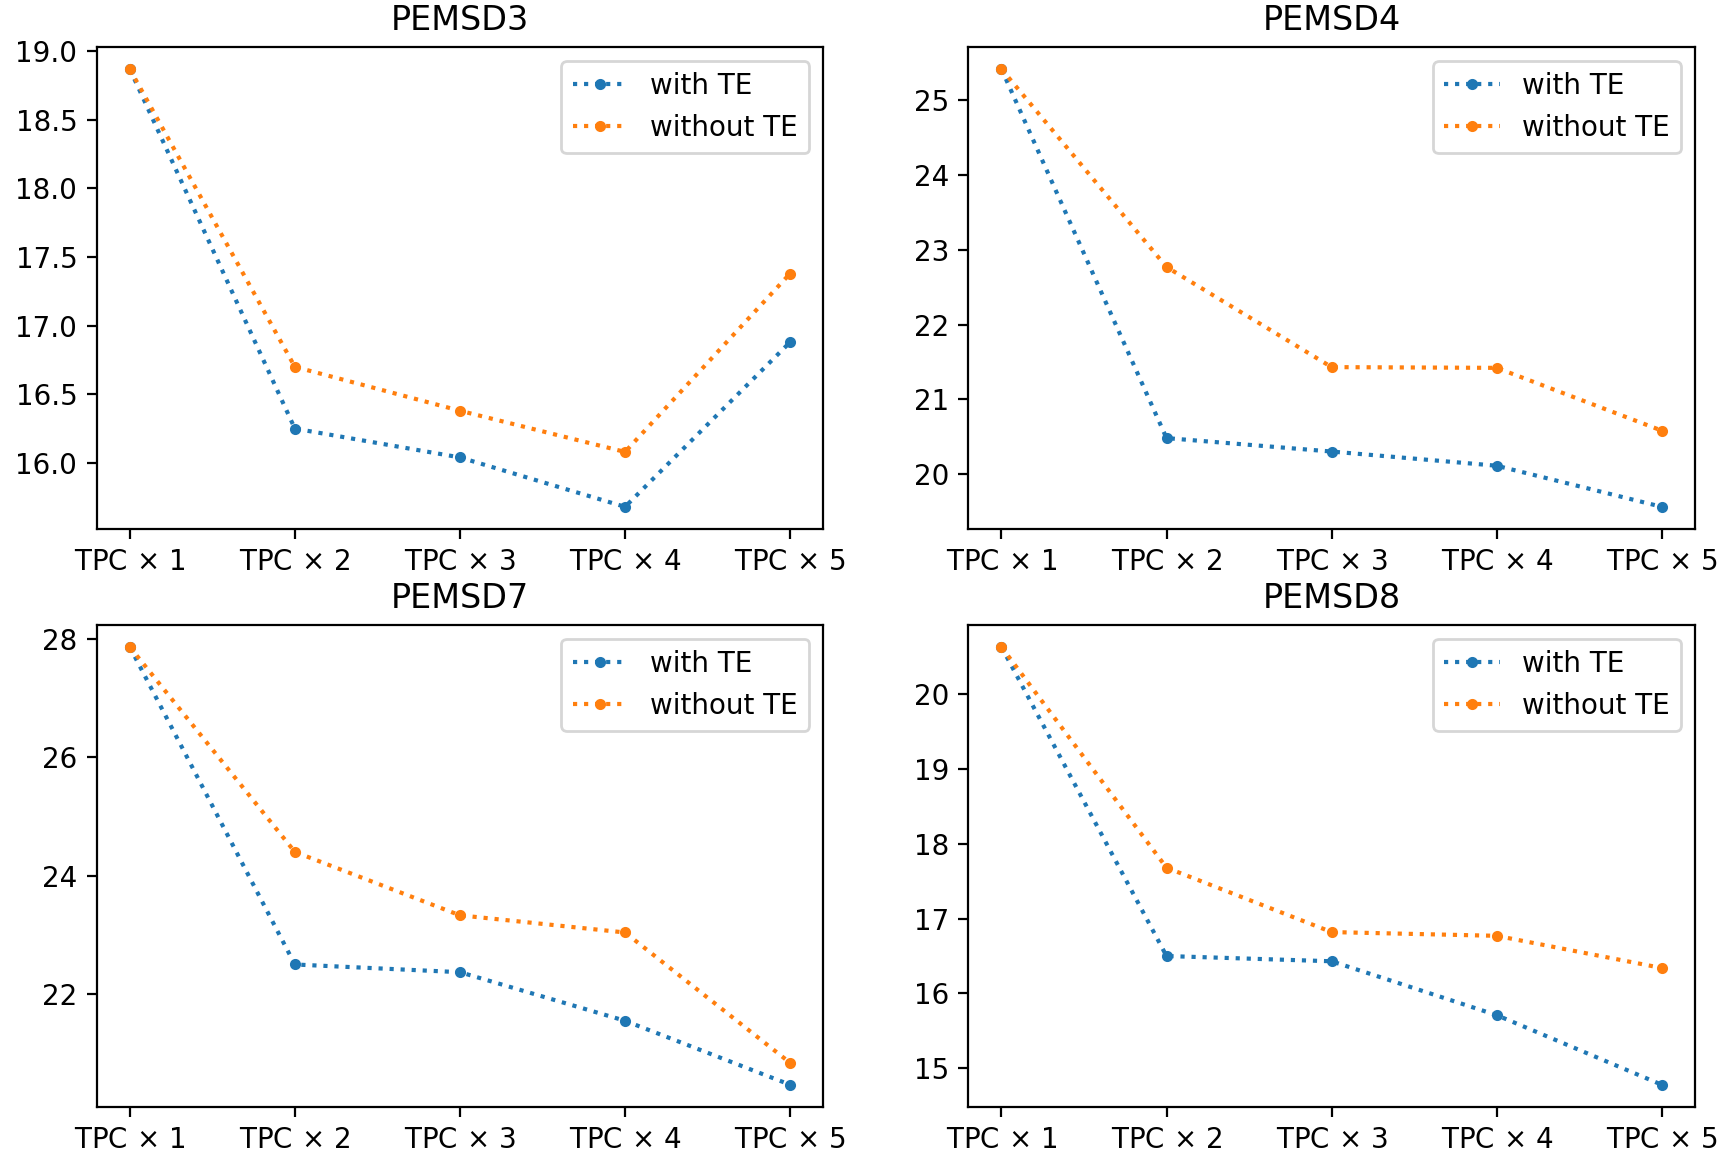
\includegraphics[width=0.48\textwidth]{pictures/Ablation.png}
    \caption{The MAE sensitivity to different settings of MS-GAT on PEMSD3, PEMSD4, PEMSD7 and PEMSD8.}
    \label{fig:ablation}
\end{figure}

First,  the multi-component structure is shown effective for spatio-temporal forecasting. Importantly, adding more components (\textit{TPCs})  to MS-GAT can contribute to accurate prediction. However, it does not mean  more components lead to the better results. As shown in Table~\ref{tab:ablation}, the model setting with four \textit{TPCs} achieves the best performance on PEMSD3, while the prediction on PEMSD4, PEMSD7 and PEMSD8 requires five \textit{TPCs} for the best. This is owing to that the traffic conditions of different physical road networks show specific spatio-temporal system complexities. When taking more historical horizons as the input of each \textit{TPC} separately, the prediction of MS-GAT would worsen instead. In other words, more input sequences to model could be harmful or meaningless. Therefore, the number of \textit{TPC} components is an important hyperparameter, which determines the performance of MS-GAT.

Second, the \textit{TE} is proven very necessary for ensuring the model accuracy. The  results in Table~\ref{tab:ablation} show the model settings with \textit{TE} are consistently superior to those without \textit{TE}. It demonstrates the traffic conditions at the past distinct time horizons have different correlation strengths with the one at the same future time horizon. Thus, the prediction effect can be significantly improved through deploying \textit{TE} in MS-GAT.

Third, the channel relation is confirmed essential for modeling the dynamics of traffic systems. The results exhibited in the last column of Table~\ref{tab:ablation} draw from the case of skipping over the channel relation when MS-GAT is under its best model setting (i.e., the one that produces the bold number in each row of Table~\ref{tab:ablation}). Clearly, when those potential channel relations coupled among traffic signals are not taken care of, the performances of MS-GAT degrade significantly. The experimental results also substantiate the effectiveness of \textit{CAttention} that applies attention mechanism to capture the channel relation of traffic signals. As a result, focusing on more interactive relations coupled within complex traffic systems contributes to improving the capability of predictive model.

\subsection{Case study}

\begin{figure}[!ht]
    \centering
    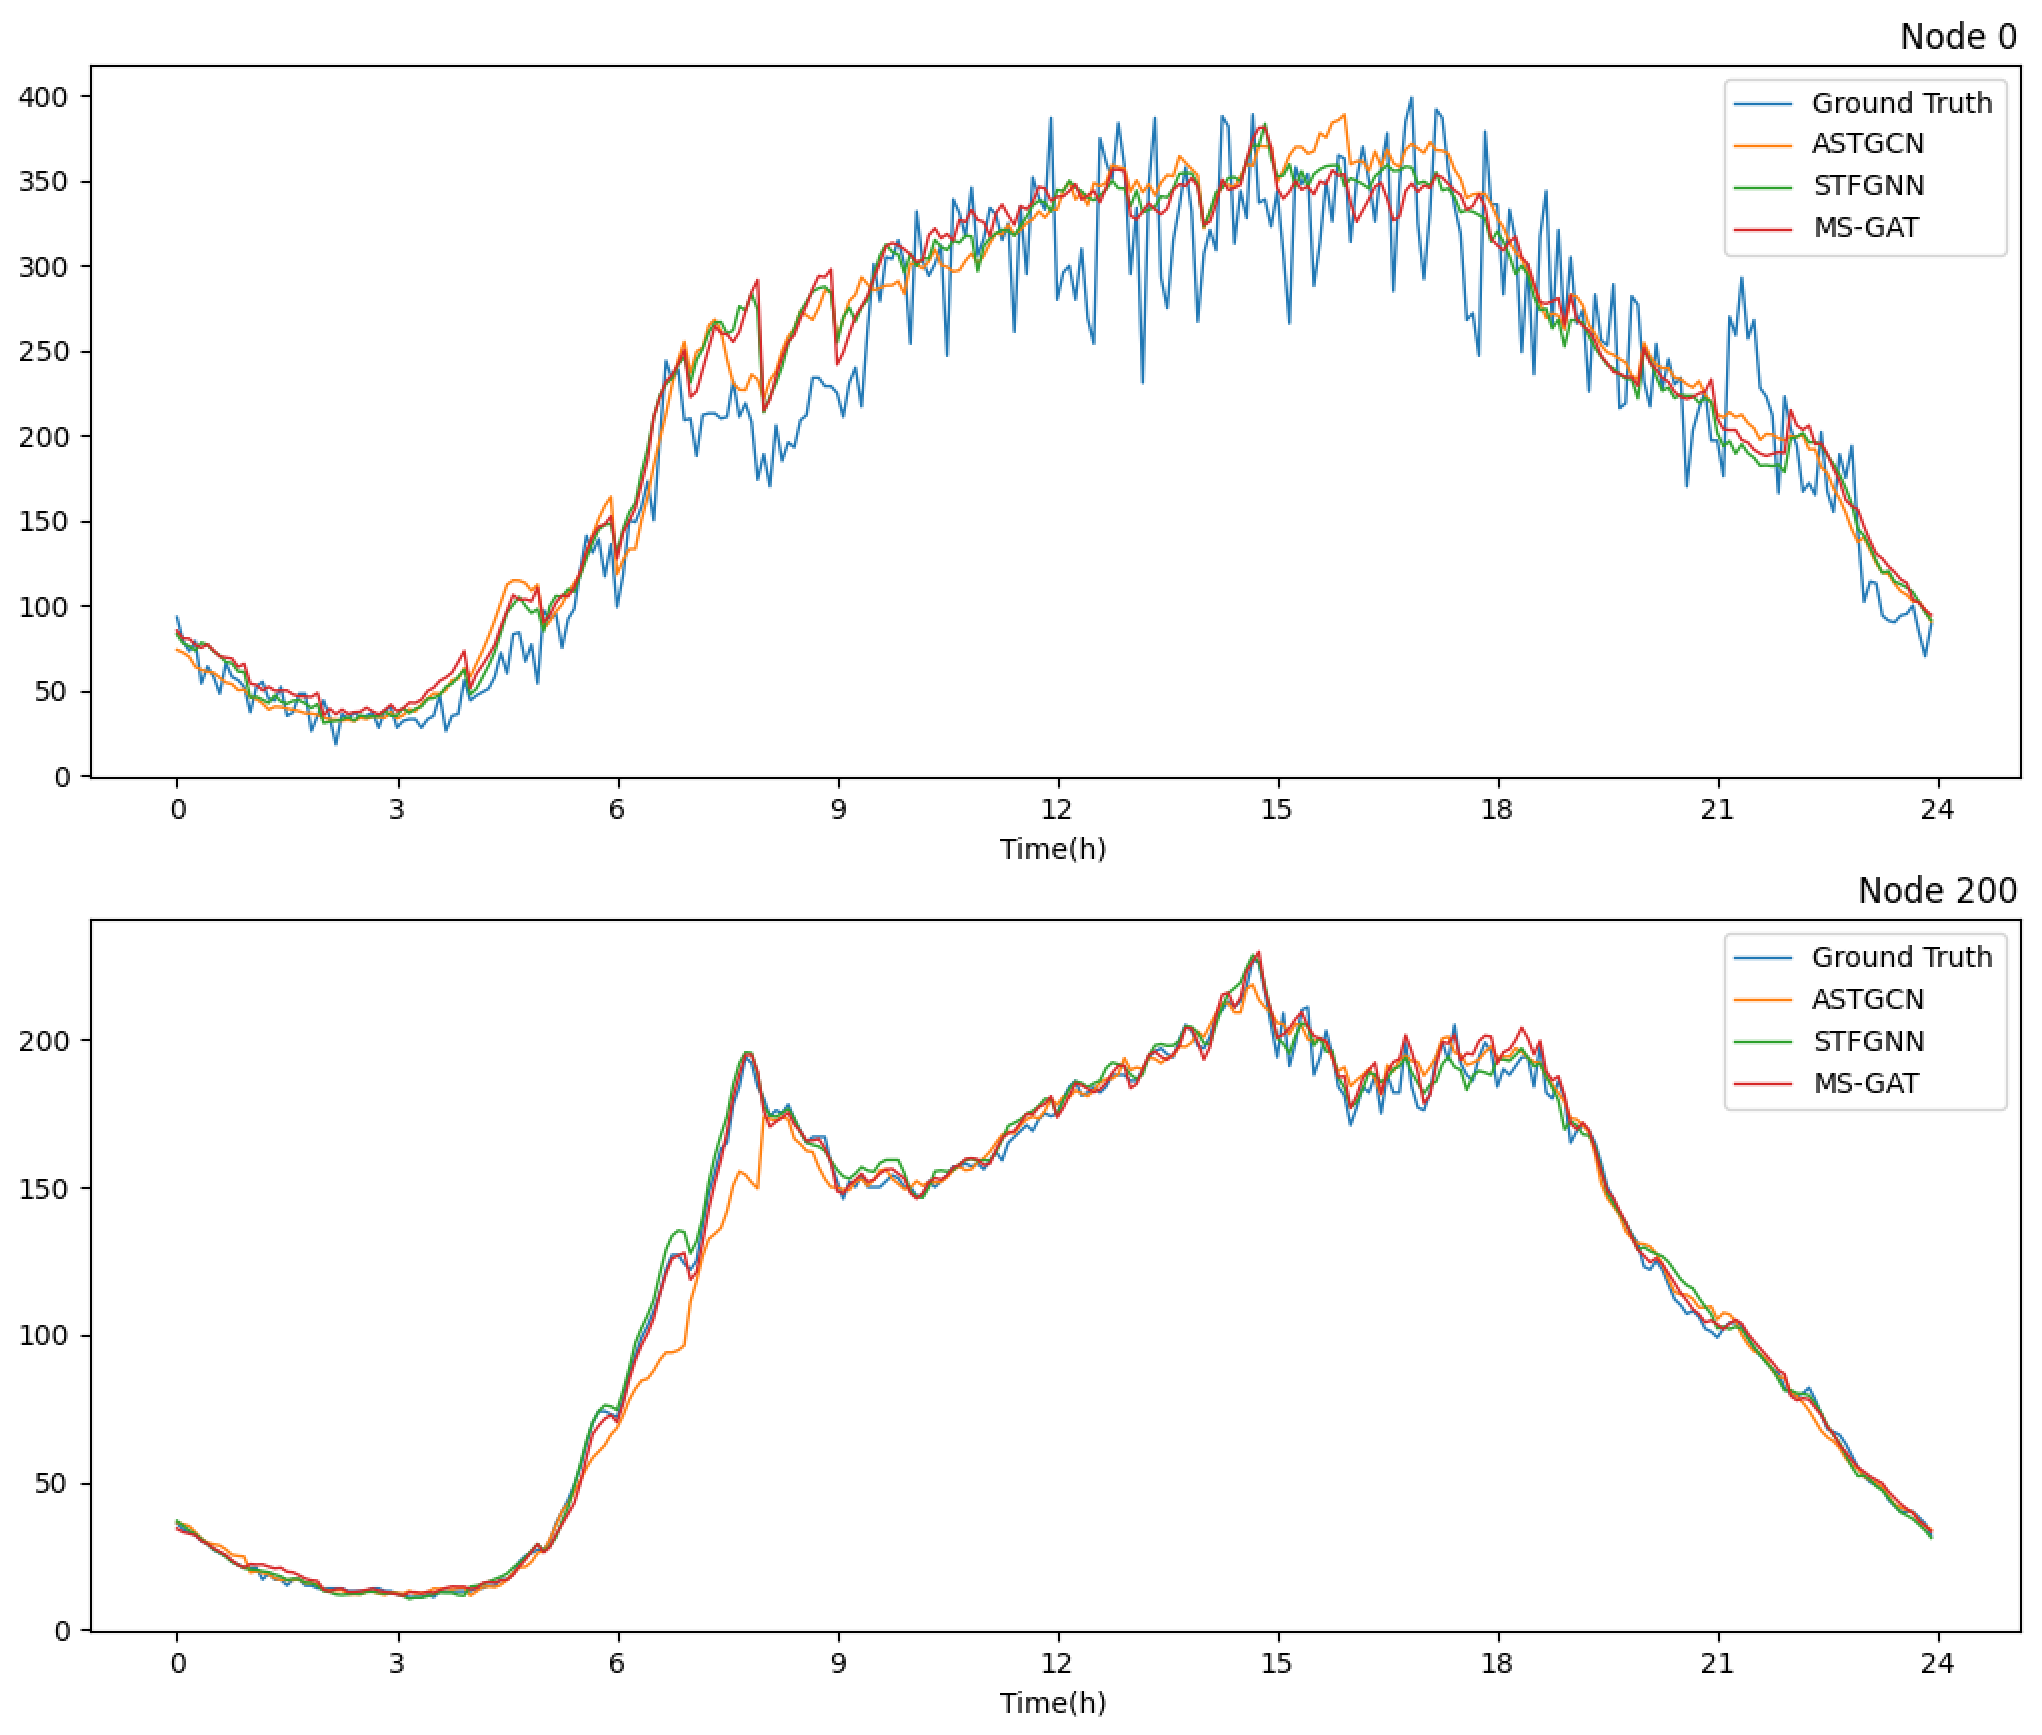
\includegraphics[width=0.48\textwidth]{pictures/Case_1.png}
    \caption{A case study of the traffic flow prediction at Node 0 and Node 200.}
    \label{fig:case_1}
\end{figure}

\begin{figure}[!ht]
    \centering
    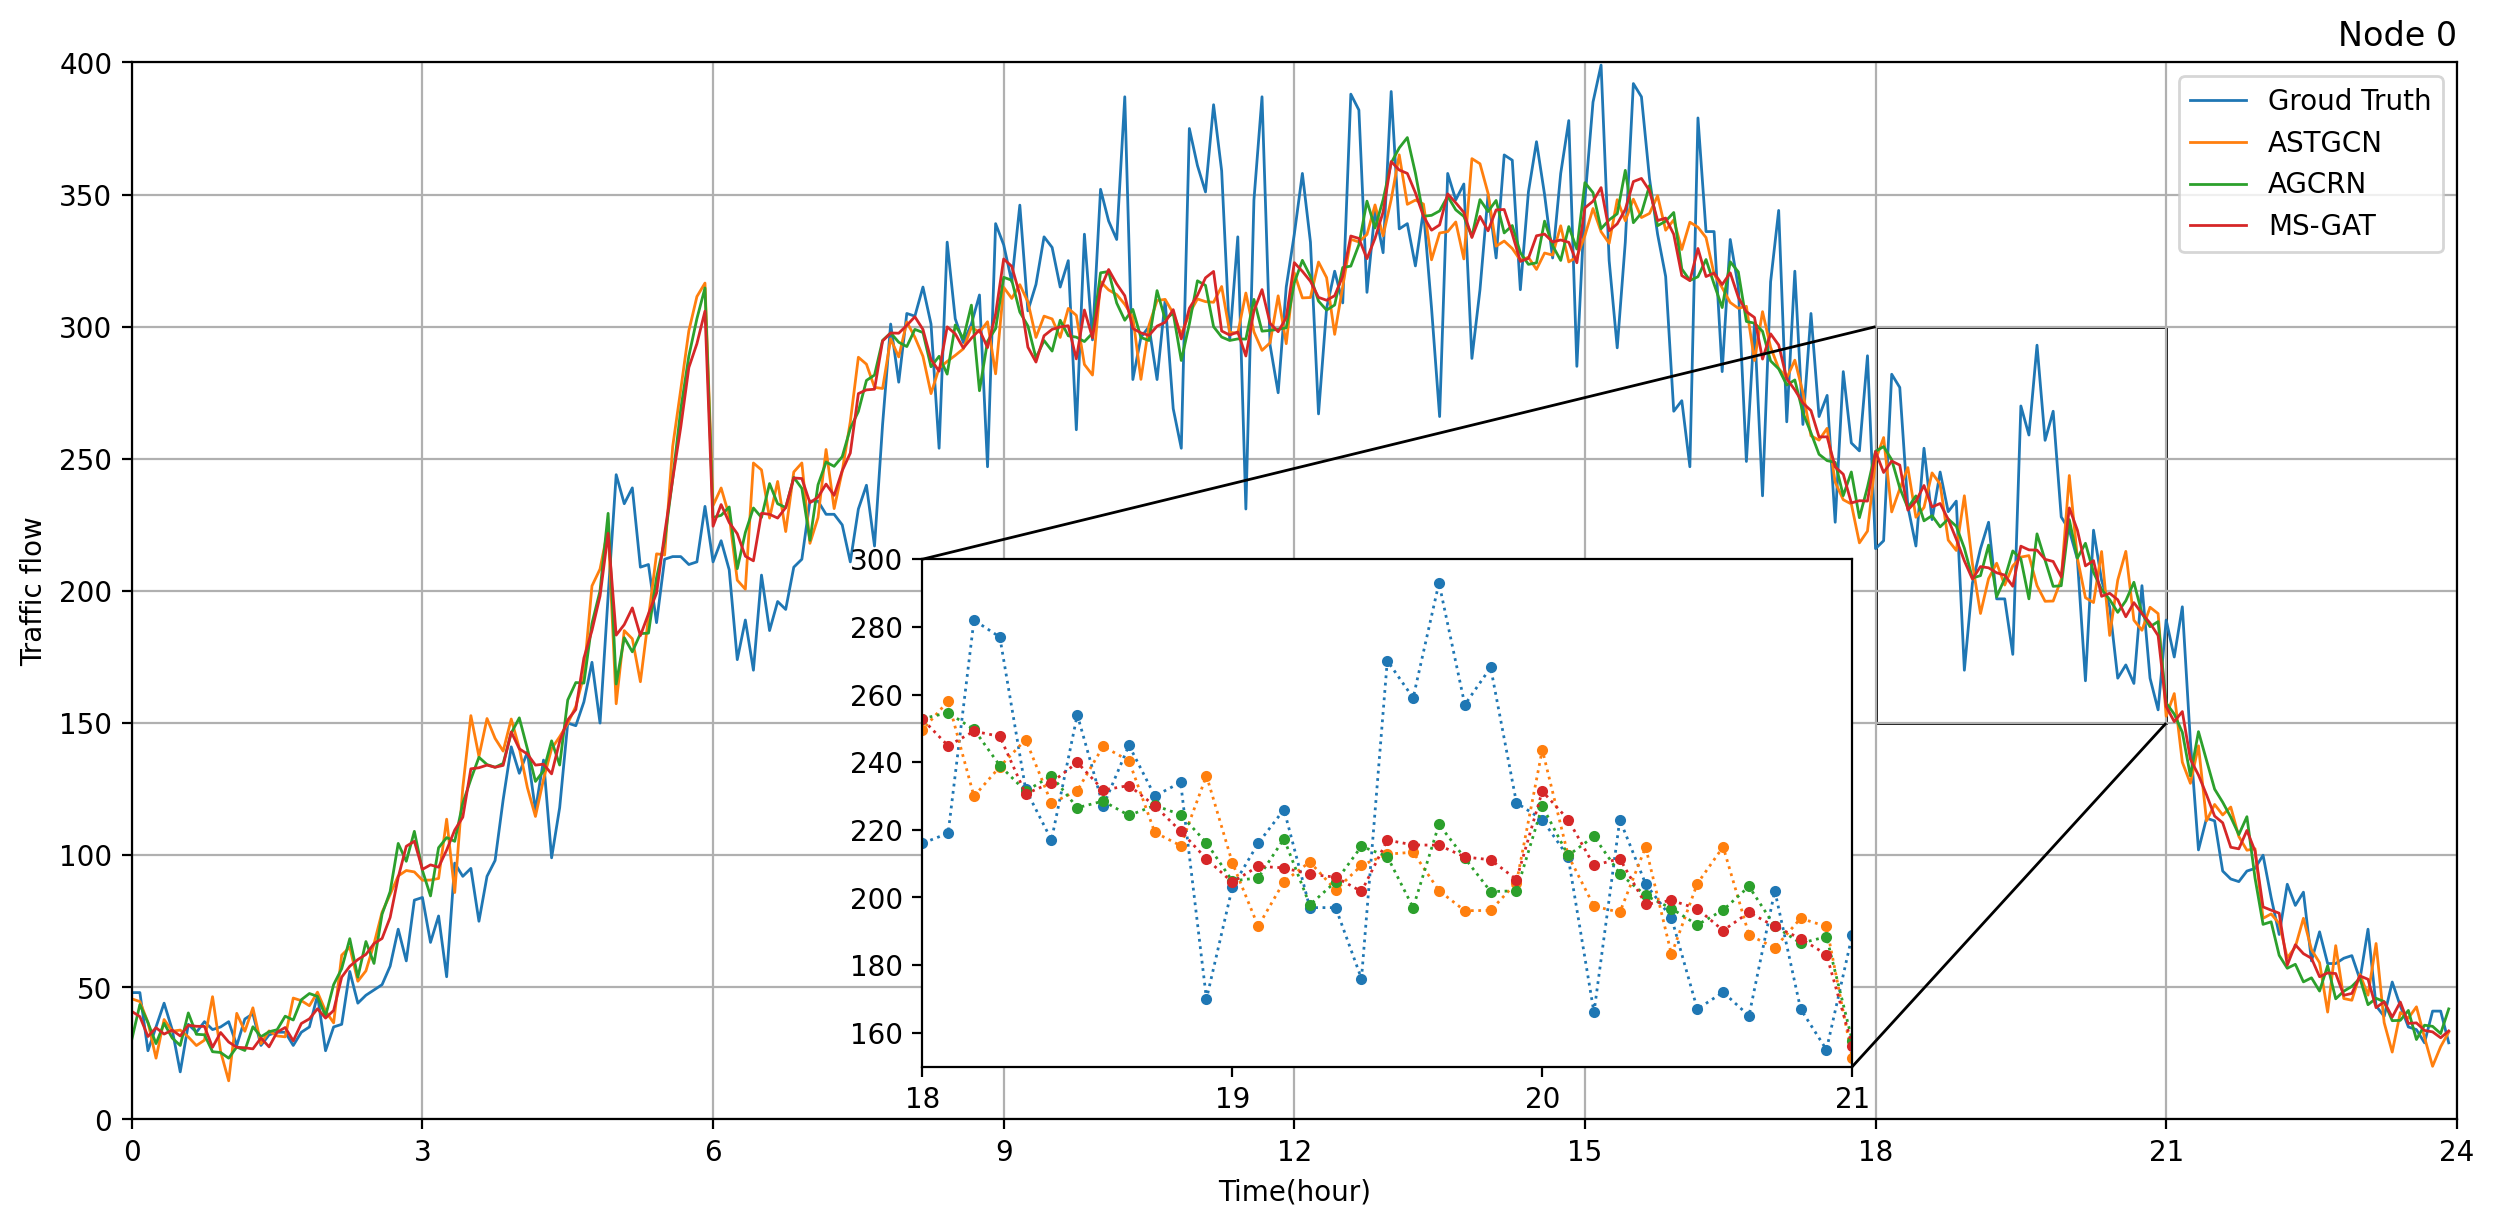
\includegraphics[width=0.48\textwidth]{pictures/Case_2.png}
    \caption{Illustration of the prediction error at Node 0.}
    \label{fig:case_2}
\end{figure}

To further investigate the performance of MS-GAT, we also conduct a case study to intuitively show its prediction effect. We select two traffic nodes Node 0 and Node 200 in PEMSD4 and plot their future 24-hour traffic flow prediction results separately in Fig.~\ref{fig:case_1} to compare two state-of-the-art models STFGNN  and ASTGCN  against our proposed MS-GAT to carry out every 1-hour interval forecasting. It can be observed that, compared to those competitive models, the prediction curves of MS-GAT on both Node 0 and Node 200 are better aligned to the temporal trends of their ground-truth traffic conditions. Fig.~\ref{fig:case_1} shows that the prediction error at Node 0 is significantly higher than that at Node 200. This is because there exist some frequent uncertain interference factors or random traffic events at Node 0 which induce the abrupt changes of traffic flow, thus exhibiting a kind of short-term recurrent blocked-unblocked traffic condition that is very challenging to be accurately estimated in practice. Fig.~\ref{fig:case_2} further shows that MS-GAT is slightly superior to the other two models, indicating that MS-GAT could adapt to such  abrupt changes of traffic conditions by its distinctive model design and parameter learning. Therefore, when performing the traffic flow prediction on the whole road network consisting of various geospatial nodes, the RMSE improvement of MS-GAT is not as significant as that in terms of MAE, which is consistent with our prior experimental results presented in Table~\ref{tab:pemsd3-8}. The reason for that is the physical road network in PEMSD4 contains many traffic nodes with short-term recurrent blocked-unblocked traffic condition like Node 0. This also triggers a future direction, i.e., further improving the stability and robustness of traffic prediction models by exploring the influence of the sharp changes of traffic conditions over nodes.


